\documentclass[letterpaper,10pt]{article}

\usepackage{titling}
\usepackage{listings}
\usepackage{url}
\usepackage{setspace}
\usepackage{subfig}
\usepackage{sectsty}
\usepackage{pdfpages}
\usepackage{colortbl}
\usepackage{multirow}
\usepackage{relsize}
\usepackage{amsmath}
\usepackage{fancyvrb}
\usepackage{amsmath,amssymb,amsthm,graphicx,xspace}
\usepackage[titlenotnumbered,noend,noline]{algorithm2e}
\usepackage[compact]{titlesec}
\usepackage[default]{droidserif}
\usepackage[T1]{fontenc}
\usepackage{tikz}
\usetikzlibrary{arrows,automata,shapes,trees,matrix,chains,scopes,positioning,calc}
\tikzstyle{block} = [rectangle, draw, fill=blue!20, 
    text width=2.5em, text centered, rounded corners, minimum height=2em]
\tikzstyle{bw} = [rectangle, draw, fill=blue!20, 
    text width=4em, text centered, rounded corners, minimum height=2em]

\definecolor{namerow}{cmyk}{.40,.40,.40,.40}
\definecolor{namecol}{cmyk}{.40,.40,.40,.40}

\let\LaTeXtitle\title
\renewcommand{\title}[1]{\LaTeXtitle{\textsf{#1}}}


\newcommand{\handout}[5]{
  \noindent
  \begin{center}
  \framebox{
    \vbox{
      \hbox to 5.78in { {\bf ECE155: Engineering Design with Embedded Systems } \hfill #2 }
      \vspace{4mm}
      \hbox to 5.78in { {\Large \hfill #4  \hfill} }
      \vspace{2mm}
      \hbox to 5.78in { {\em #3 \hfill} }
    }
  }
  \end{center}
  \vspace*{4mm}
}

\newcommand{\lecture}[3]{\handout{#1}{#2}{#3}{Lecture #1}}
\newcommand{\tuple}[1]{\ensuremath{\left\langle #1 \right\rangle}\xspace}

\addtolength{\oddsidemargin}{-1.000in}
\addtolength{\evensidemargin}{-0.500in}
\addtolength{\textwidth}{2.0in}
\addtolength{\topmargin}{-1.000in}
\addtolength{\textheight}{1.75in}
\addtolength{\parskip}{\baselineskip}
\setlength{\parindent}{0in}
\renewcommand{\baselinestretch}{1.5}
\newcommand{\term}{Spring 2014}

\singlespace



\begin{document}

\lecture{ 33 --- Software Communication Patterns}{\term}{Jeff Zarnett}

\section*{Software Architecture, Continued}
In this lecture, we are going to look at software architecture, but from a different perspective. In the last lecture we considered how to architect a piece of software. This time, we will examine some different communications architectures: how messages and data are passed from one system or part of a system to another.


\subsection*{Pipes and Filters Architecture}
A pipes and filter architecture, as the name suggests, has two major components: pipes and filters. A pipe, quite simply, takes some input, performs some action on the data, and then outputs the result. Pipes take one input, are supposed to do one small thing only (and do it well), and produce one output. A filter examines the data it receives as its one input and will either accept it (let it pass and appear in the output) or reject it (block it and no output appears). 

Suppose some input messages are formatted with CRLF (Carriage Return + Line Feed) characters at the end of each line. This data will be sent to a system that recognizes only LF (Line Feed) characters as the end of line and considers CR (Carriage Return) to be an error. Solution: create a pipe that removes the CR characters. Messages then pass through the pipe, and if they have CRLF line endings, the pipe removes the CR characters, leaving just the LF. The system on the other end will then function the same way whether the original message has CR characters or not.

This is not the only option, however: a filter might work here as well. Instead of a pipe that removes CR characters, create a filter that checks for CR characters and rejects the message if they are found. The rejected message does not proceed and it is not delivered to the system that considers CR to be an error.

Pipes do not necessarily have to transform data; it might only read data. You may have a pipe that just logs data (message reference numbers, date and time, sender and recipient, et cetera). Filters, however, are always read-only: they do not change the data at all.

Any combination of pipes and filters can be assembled to form a \textit{pipeline}. Data enters at the start of the pipeline, and passes through the pipes and filters until it gets to the end of the pipeline. Each pipe does one function to the data. Filters may be inserted at any point in the pipeline, and if a filter blocks a piece of data, it proceeds no further in the pipeline. Thus, a more complex system is built up by assembling many smaller components in the correct order. Because individual components are small, they can be easily combined in whatever way is appropriate.

One major advantage of this system is that the individual elements (pipes and filters) are small and simple, and can often be re-used. Because the pipe or filter does exactly one thing, it is easy to test and verify its operation. As disadvantages, these systems often have many interacting components and changes in one pipe might affect many pipelines, and the pipes and filters model does not work very well in systems where there is a need for a lot of decision-making later on in the process about what path the data should follow.

Some advanced pipe-and-filter systems have a third element called a \textit{valve}. Unlike pipes, which have exactly 1 input and exactly 1 output, or filters, which have exactly 1 input and either 0 or 1 output, the valve takes one input but has 1 or more outputs. This can be used to decide farther down the pipeline, what path a message should take. For example, based on the recipient of a message, you might send it either by e-mail or by instant message.

\paragraph{Example.} We have a system that accepts XML data within a ZIP file and delivers the extracted XML to a server. A pipeline for such a system might be written like this:

validZIPFileFilter/extractFromZIPFilePipe/loggingPipe/removeCRPipe/syntaxFilter/deliverToServerPipe\\

The slashes (/) indicate the separation between the different segments of the pipeline. This example has four pipes (extractFromZIPFilePipe, loggingPipe, removeCRPipe, deliverToServerPipe), and two filters (validZIPFileFilter, syntaxFilter). It's not (usually) a requirement that pipe names end with -Pipe and filter names end with -Filter, but it is a nice practice to make it clear which is which. Below, a short description of what each part does:

\begin{itemize}
	\item \textbf{validZIPFileFilter} - Rejects any input which is not a valid ZIP file.
	\item \textbf{extractFromZIPFilePipe} - Extracts the data from the ZIP file. At this stage we can be sure that we have a ZIP file as the input (and not a plain text or pdf file or something else) because those would have been blocked at the previous stage.
	\item \textbf{loggingPipe} - Examines the extracted data and writes some information to the logs. 
	\item \textbf{removeCRPipe} - As above, removes the Carriage Return characters from the data, if any.
	\item \textbf{syntaxFilter} - Accepts only data which has valid syntax (XML is valid); rejects all others.
	\item \textbf{deliverToServerPipe} - Sends its input to the server via some specified form of communication.
\end{itemize}

\paragraph{UNIX Example.} UNIX and UNIX-like operating systems use some concepts from the pipes-and-filters architecture. The system utilities like \texttt{ls}, \texttt{cat}, and so on are all small and do exactly one thing. On the commandline you can create a pipeline connecting these two or more items. Here's a UNIX command:

\texttt{cat lectures.txt | grep blackboard}

This is actually two different commands linked together in a pipeline. The first command, \texttt{cat}, reads the file \texttt{lectures.txt} and outputs it. If that command were run alone, it would output the text of the file to the console, but instead there is a \texttt{|} pipe symbol after it, which means the output of the \texttt{cat} command is piped to the \texttt{grep} command. The \texttt{grep} command searches its input for occurrences of the word ``blackboard'' and prints as output the lines where the word blackboard is found. Because we did not specify another pipe symbol and another destination, the output of \texttt{grep} appears on the console.


\subsection*{Blackboard Architecture}
In a blackboard architecture, there exists a common knowledge base, called the ``Blackboard'', and a set of independent agents work on the knowledge base, each updating it with partial solutions. These agents co-operate and solve the problem.

The name comes from a simple metaphor: imagine you have a very difficult math problem and you have assembled a group of excellent mathematics professors in the room. To arrive at a solution, the professors will collaborate on the blackboard. They start with a problem statement and each professor looks at the blackboard and watches for an opportunity to apply his or her expertise. When one writes something new on the board, each professor takes a look and sees if he or she can contribute now. If so, he or she will then apply his or her knowledge and write the result on the board. This will hopefully trigger another professor to be able to do something with that, and the professors will continue adding their contributions to the blackboard until the problem is solved (or until nobody can proceed, in which case, they have failed to solve the problem).

A blackboard system has three major components. The first is the software agents, sometimes called ``Knowledge Sources''. These are the agents (professors) of the system. There is also the blackboard, the shared repository of problems and partial solutions; this is the input to and output from the agents. The final element is the moderator that controls the flow of access to the system so that the agents do not interfere with one another. To extend the metaphor, the moderator stands at the front of the room and prevents the professors from fighting over the chalk or accidentally overwriting another's work~\cite{blackboard}.

This is an unusual software architecture and there are very few problem domains where this is the best choice; usually there is only one agent or there are multiple agents, one of which is best able to handle the problem. One of the more common examples is optical character recognition (OCR). In OCR, we have a document in print form and we want to scan it in to the computer, but not just as a picture; we want to extract the text (to the extent that this is possible). Another major domain is using this in artificial intelligence systems~\cite{blackboard2}.

One potential advantage is that it might be possible to solve problems this way that would otherwise not be solvable, or they could be solved faster, more efficiently, or better than any individual agent could accomplish. The disadvantages are that the systems are complex at best, difficult to understand, and only applicable to a small number of problem domains.


\subsection*{Publish-Subscribe Architecture}
In the publish-subscribe architecture, communication takes place by passing messages. The sender of a message is called a \textit{Publisher}. The publisher does not know whom the reciever(s) of the message is (are). On the other side, receivers, called \textit{Subscribers}, register their interest in certain kids of messages without knowledge of any publishers.

There may be a third party involved, called a \textit{Broker}, whose job it is to connect the publishers and subscribers indirectly. If there is no Broker, any subscriber who is not ``listening'' at the time the message is published will not receive the message. The broker is a place where the publisher can publish the message such that subscribers can collect the message at their convenience.

It is rare for any subscriber to be interested in all kinds of messages. There are two major ways to filter these messages so a receiver only gets the ones of interest. These solutions are not mutually exclusive; both can be employed in the same system.

\textit{Topic-Based} systems have a list of topics, and publishers write in these topics (broadcast on this channel) and subscribers listen to that channel. Example: I create an ECE~155 topic, and students subscribe to it. It is then my responsibility as the sender to identify a message in advance as being part of the ECE~155 topic so it will be published on that channel. 

In a \textit{Content-Based} system, messages are delivered to a subscriber if the content of that message matches what the subscriber is looking for. Continuing the example from above, a student might put as the desired attributes that the text contains, somewhere, ``ECE~155''. Any message sent out that matches the criteria of the receiver will be delivered to the receiver.

There are some advantages to this architecture. The first is that there is limited dependency between publishers and subscribers. In a client-server architecture, the client cannot send messages to the server; in publish-subscribe, the publisher can send messages to the broker (if one is available) even if no subscribers are ready yet; similarly, if the publisher system is down, receivers can get their messages from the broker. This architecture also scales well, since we can have $n$ publishers and $m$ subscribers.

There are some disadvantages in that we may not be certain that a message has been delivered successfully. The publisher may assume that subscribers are listening even if they are not. Also, the broker might be a central point of failure.

The most common example of publish-subscribe is likely something you are already familiar with: RSS feeds. RSS (Really Simple Syndication) works on the publish-subscribe model. The author of something, such as a blog post, publishes his writing on the blog. Anyone who is subscribed to the RSS feed gets a notification that a new message has appeared. This new message contains the published content.

\subsection*{Peer-to-Peer Architecture}
A peer-to-peer (P2P) system is one in which the different nodes (computers or programs) in the network both supply and receive resources, in contrast to the client-server model where the client requests some resources that the server provides. Tasks like searching for files or streaming audio/video are shared amongst the interconnected peers, who contribute some resources (processing power, network bandwidth) to other participants without a centralized server~\cite{p2p}.

Some P2P systems, as shown below, do have a central node that is used as an indexing or registration service, to help peers find one another.

\begin{center}
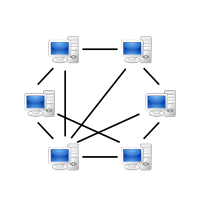
\includegraphics[width=0.35\textwidth]{images/p2pnetwork.png}
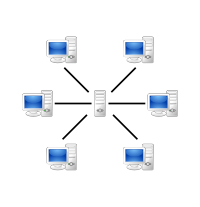
\includegraphics[width=0.35\textwidth]{images/serverbased.png}\\
Left side: A P2P network with a central admin system;\\
Right side: a network based on the client-server model.\\
\texttt{http://en.wikipedia.org/wiki/Peer-to-peer}
\end{center}

As you might have noticed, peer-to-peer systems became very popular starting in 1999 with Napster. Napster was a peer-to-peer file transfer system, used to share music. There was no central repository of music files; instead each user shared what files he or she had locally with others and could browse the files others made available themselves. Although P2P systems are commonly associated with the sharing of copyrighted material (music, movies, et cetera), the P2P network is just the form of communication and is content-agnostic. Linux distributions like Ubuntu often provide an option to download their installation CDs via BitTorrent (a P2P protocol).

The major advantage of P2P networks over the traditional client-server model is that their ability to serve content increases as more requests come in rather than decreases. A traditional server can handle only so many concurrent requests before performance is compromised or it cannot accept any new requests. 

The biggest disadvantage is the amount of work that needs to go in to the network's communication and searching. As networks of nodes can be unstructured, it is difficult to search and find anything. The way to search is to send and receive a lot of data as different peers are asked repeatedly for their results. Even with all that traffic, the searcher might not find what he is looking for, even if there is a peer who is sharing that resource. There is also a lot of data sent and received to communicate about peers entering or leaving the network, which can happen frequently~\cite{p2p2}.

(If peer-to-peer networks are a subject of interest for you, take the class ``Distributed Systems''.)

\bibliographystyle{alpha}
\bibliography{155}


\end{document}